\chapter{Related Work}
\setcounter{section}{0}

This chapter will hold the parts of the project coming from the outside, all the relevant efforts happening in the Solid Community or \gls{cern}'s involvement in the collaboration.

\section{Background}

The \textit{\gls{cern}-Solid Code Investigation} project aims at linking \gls{cern} with Solid. Some of this linkage has been done in the form of a status quo check of the Solid ecosystem in \cite{cern-solid-investigation-spec}. This previous work and the efforts around the two \glspl{poc} shall give insights into a symbiosis of \gls{cern} and Solid.

The following sections in this chapter will introduce the two systems and their significant subsystems, modules, libraries, or techniques. 

\section{Indico}

Indico is one of CERN’s most sophisticated software projects. It is an event management tool, giving users a means to organize complex meetings or conferences with an easy-to-use interface. It was started in 2002 as a \textit{European project} and has been in production at CERN ever since. It is used daily to facilitate more than 600,000 events at CERN. It has helped others like the UN “to put in place an efficient registration and accreditation workflow that greatly reduced waiting times for everyone” at conferences with more than 180,000 participants in total \cite{cern-solid-investigation-spec}.

\subsection{Events}

Being an event management tool at Indico's core lies the \texttt{Event} class. The Event's user interface is presented in \ref{fig:indico-event-interface}, showing all sorts of attachable information. 

\begin{figure}[H]
    \centering
    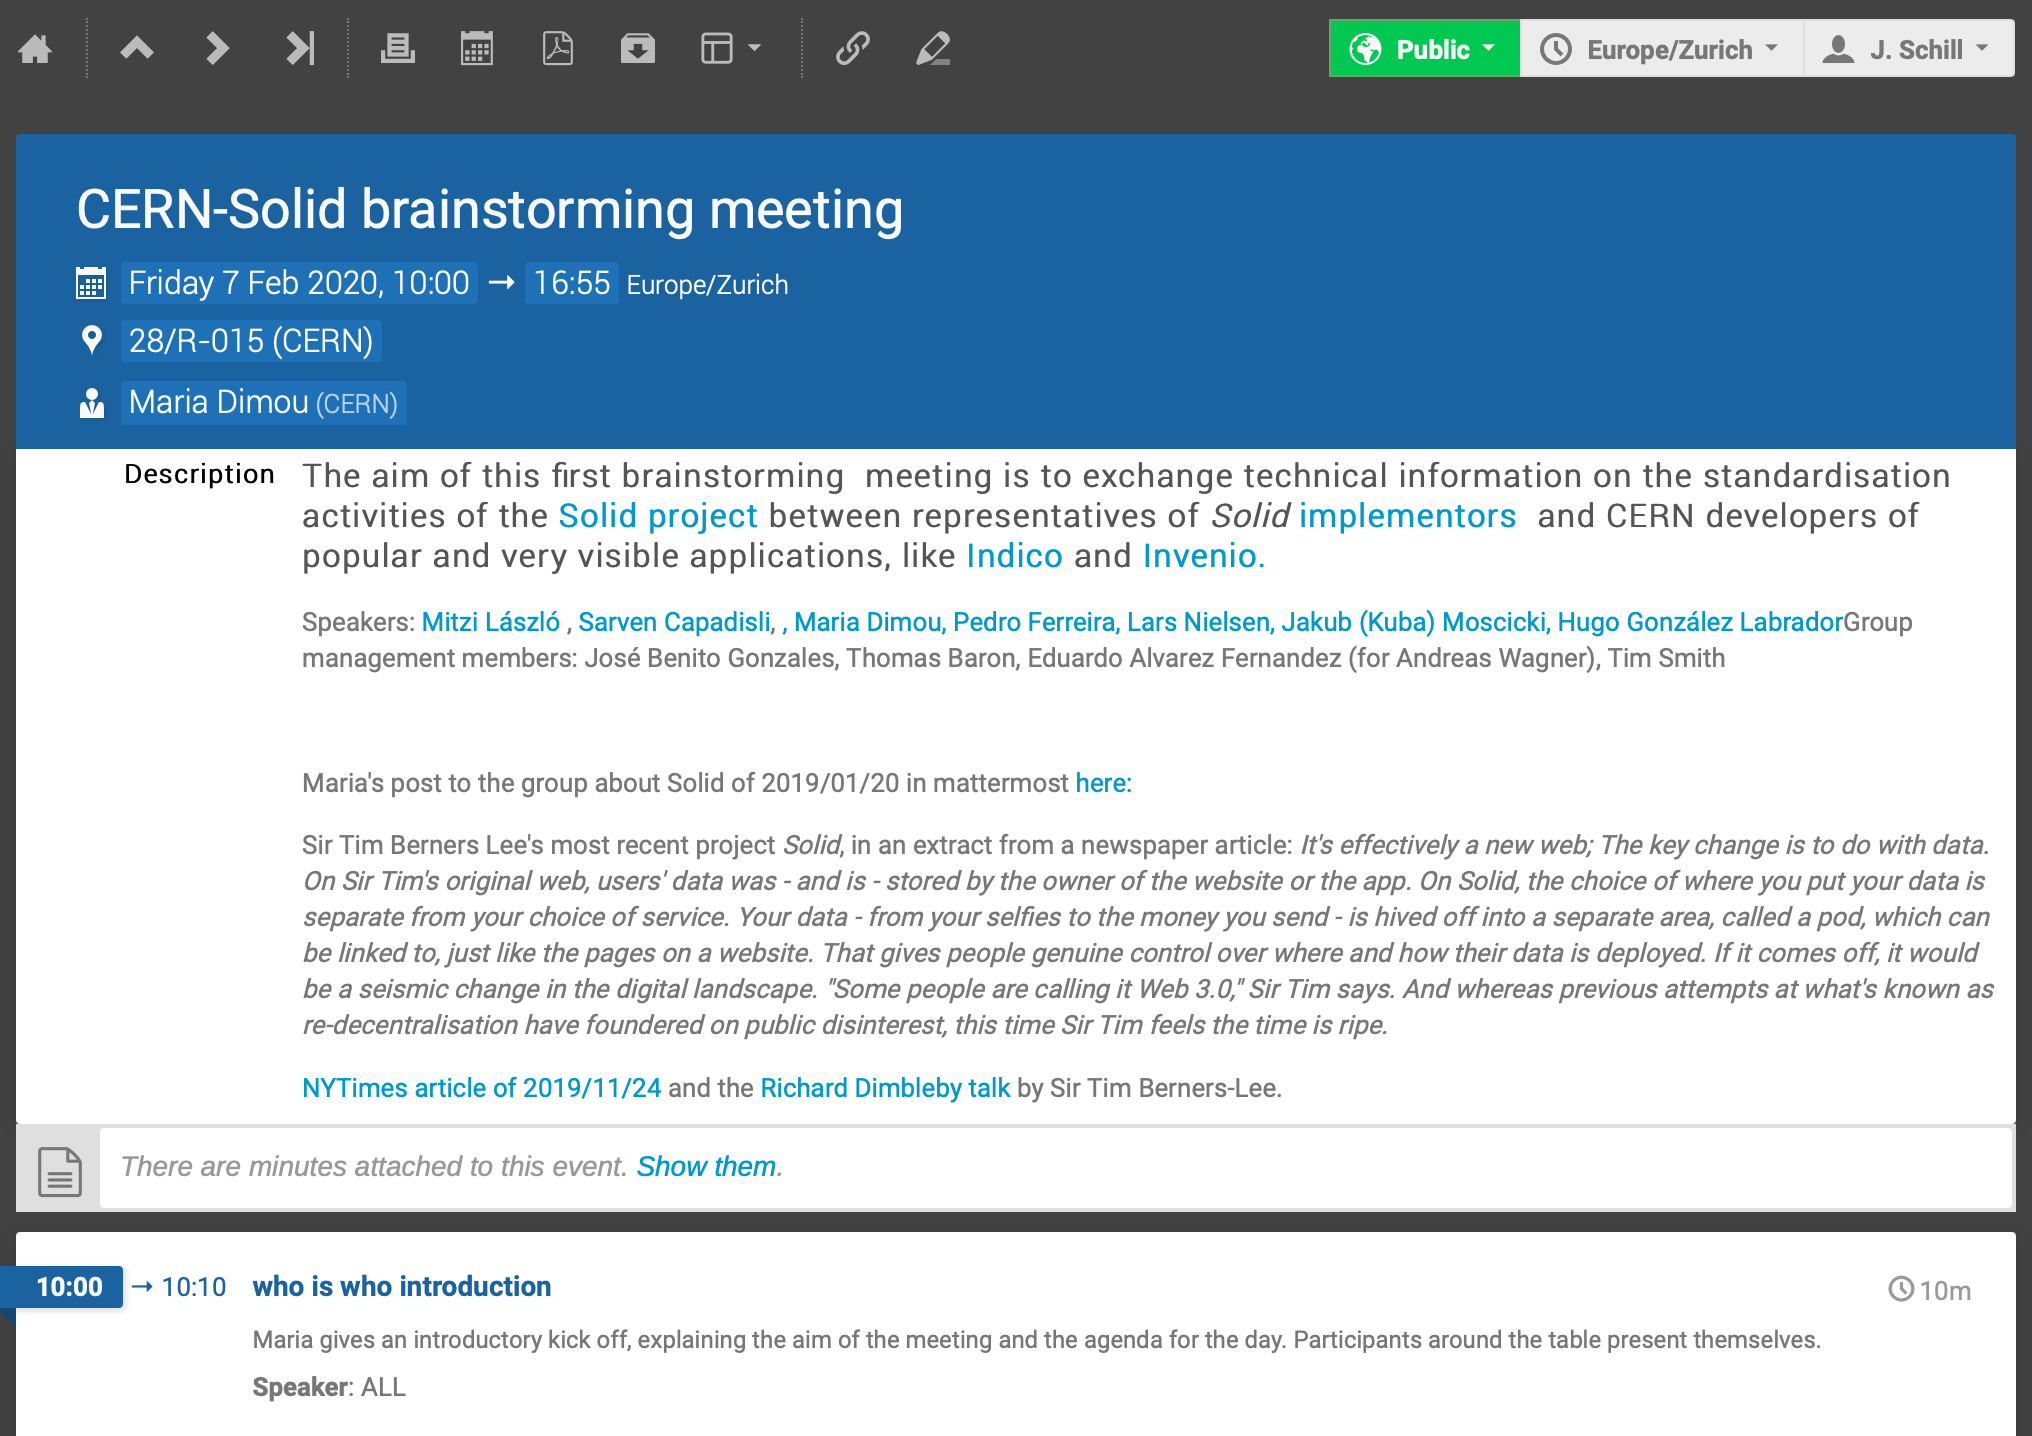
\includegraphics[width=0.6\textwidth]{thesis/latex/assets/indico-event-interface.png}
    \caption{User interface of an Indico event.}
    \label{fig:indico-event-interface}
\end{figure} 

\subsection{Storage Mechanisms}

All events, all information in these events, file uploads, everything put into Indico are stored in a relational database on centralized servers. \gls{cern}'s Indico instance is hosted on-premise in their own data centers. Another crucial feature of Indico is the permanent archival of event material and metadata \cite{cern-indico}. It allows the lifetime access to all events hosted on the platform. As an example one can easily browse to the event "Big Data and Social Media" held by Vint Cerf in 2018 \cite{vint-cerf} and have access to description, recording, and slides, or even a presentation given in 2004 about "Practical Use of XML" \cite{titov}.

\subsubsection{EventSettingsProxy}\mbox{}\\

A \textit{proxy class} enables storage for event-specific settings. Commonly stored data types are contact email addresses for an event. In Indico these \texttt{EventSettingsProxy} are stored in a database table called \texttt{settings}. Adding a new setting for the \gls{poc} it will receive a field in the row specific to the event.

\subsection{Conferences}

In Indico, an event can be simple meetings, lectures, or all kinds of presentations. Additionally, Indico allows the creation and management of conferences. Conferences are more complex events with several more features, including registration, call-for-abstracts, program definition, payments, and more \cite{cern-indico-docs}. The conference registration is especially interesting for this project as it is part of the \gls{poc}.

\subsubsection{Conference Registration}\mbox{}\\

Once a conference is created, the conference manager needs to make a registration form to allow signups to the event. This form is created in Indico's backend and has default personal information fields but can be expanded as much as needed with free text fields. Payment for participation also needs to be enabled in this step. Meaning, as soon as a user fills in all the mandatory information and submits it, a successfully finished payment prompt will only complete the registration.

\section{Solid}

A initial introduction to Solid was given as part of a previous \textit{research project} \cite{cern-solid-investigation-spec} in preparation for this thesis. In the \textit{research project}, the Solid specification was, among other things, summarized and analyzed. This section will reiterate and study the subsequent experiment-relevant parts further.

\subsection{Authentication With Solid}

In the Solid ecosystem, agents identify themselves with their WebID and prove their ownership through the \gls{solidoidc} protocol, which is a flavor of \gls{oidc}. For further explanation and flow diagrams through the authentication process, see either the work done in the previous report \cite{cern-solid-investigation-spec} or the \gls{solidoidc} specification itself \cite{solid-ecosystem-oidc}.

To help with the complex authentication flow of \gls{solidoidc} a few libraries have been developed by different actors. Two libraries relevant for this project exist; their relevancy is discussed in the chapter \ref{chapter:investigation} under the section \ref{subsubsection:design}.

\begin{table}[h!]
    \centering
    \begin{tabular}{| l | l | l |} 
     \hline
     Name & Solid Auth Fetcher & solid-client-authn \\
     \hline
     Repository URL & \url{github.com/solid/solid-auth-fetcher} & \url{github.com/inrupt/solid-client-authn-js} \\
     \hline
     Language & \gls{ts} & \gls{ts} \\
     \hline
     Maintainer & Solid Community & Inrupt \\
     \hline
     Last updated & 2021/03/05 & 2021/05/12 \\
     \hline
    \end{tabular}
    \vspace{0.75cm}
    \caption{Two Solid authentication libraries.}
    \label{table:0}
\end{table}

Solid Auth Fetcher is a fork of the \texttt{solid-client-authn} developed by Inrupt but has not seen much development in recent time. With the quickly evolving Solid ecosystem, it is vital to have working and up-to-date libraries to build applications in this ecosystem. Both libraries do not differ in their core functionality, and both support authenticating with the latest Solid servers, and thus the choice is not as important. Still, the frequency of commits in Inrupt's repository seems to indicate a more active development and a more reliable source when problems arise. This way, one does not rely on support from open-source developers, which is, per se, not a bad thing.

For this simple reason, the programming of the \gls{poc} where Solid authentication was needed was enabled through Inrupt's \texttt{solid-client-authn}.

\subsection{Reading and Writing Linked Data}

Data in Solid is stored as Linked Data \cite{Malhotra:15:LDP}. \gls{rdf} is a framework for representing information of Linked Data in the Web \cite{Cyganiak:14:RCA}. The default file format so far implemented by the existing Solid servers is \textit{Turtle} \cite{Prud:hommeaux:14:RT}.

The graph-based data model from using \gls{rdf} also requires additional computation as it is not natively supported with helper functions in \gls{js}, such as \gls{json}. The benefit of using \gls{json} in \gls{js} is that a \gls{json} object is automatically parsed as an object and can be operated on by using the dot notation to access attributes of the \gls{json} data structure. For \gls{rdf}, this is not the case for an into the program loaded Turtle resource.

Fortunately, existing libraries come to the rescue allowing such operations on the \gls{rdf}-based data type. Again Inrupt and the Solid Community offer solutions. Again, Inrupt's solution was chosen for this development as it acts as a convenient wrapper to the bare bone Linked Data \gls{api} implemented in \texttt{rdflib.js} \cite{rdflib-js}. Even though working with \gls{rdf} can be quickly done with just using \texttt{rdflib.js}, Inrupt's libraries tie nicely together and allow for instance a seamless passing of an authenticated session to its client library to enable authenticated requests to protected resources.

As mentioned before and looked at in detail in \cite{cern-solid-investigation-spec}, the Turtle format is a graph data structure built-up with triplets---a triplet statement in its simplest form a sequence of (subject, predicate, object) terms \cite{Prud:hommeaux:14:RT}. 

Inrupt decided to call this construct a \texttt{Thing}, which is a data entity associated with a set of data or properties of this \texttt{Thing} \cite{inrupt-thing}. A \texttt{SolidDataset} is a set of things \cite{inrupt-dataset}.

The following code listing shows how the helper methods can be used to extract data from a Turtle file loaded by a request to the WebID profile document \gls{uri}.

\begin{lstlisting}[language=Other,columns=fullflexible, caption={Basic usage of Inrupt's solid-client library.}, label={lst:2}]
// Import statements omitted for this demonstration
// 1
const myDataset = await getSolidDataset(
  "https://janschill.net/profile/card"
);
// 2
const myProfile = getThing(
  myDataset,
  "https://janschill.net/profile/card#me"
);
// 3
const fn = getStringNoLocale(myProfile, VCARD.fn);
// fn => "Jan Schill"
\end{lstlisting}

\begin{enumerate}
    \item \textbf{Fetching the Turtle resource at the given \gls{uri}}: Notice here the WebID profile document \gls{uri} is being loaded, which refers to the document describing the agent behind the WebID \gls{uri}.
    \item \textbf{Loading triplet statement into variable}: Now, the actual triplet statement containing information behind this specific agent is mapped to the \texttt{myProfile} variable.
    \item \textbf{Reading a value from a triplet}: Every subject and predicate is a \gls{uri}. The subject here is the loaded profile from the WebID \gls{uri} and the to be extracted value from the statement matching on the subject and predicate. The predicate \texttt{VCARD.fn} when evaluated returns a \gls{uri}, which on dereferencing describes what kind of value can be obtained from the object.
\end{enumerate}

\subsection{Authorization Through WAC}

The as per Solid specification decided authorization mechanism is through \gls{wac} \cite{wac}. The majority of Solid servers use \glspl{acl} to manage the access modes on containers and resources.

TODO: more here

\subsection{Application Launcher}

A so-called \textit{application launcher} can mitigate a later presented discovery of a flaw in assigning unnecessary full access controls. The inconvenience lies in the fact when an application asks the client for what the allowed scope to its data pod is, most often, complete access control on the root container is needed -- this is against the security principle or tactic called \textit{least privilege}. The least privilege means to give actors of a system only exactly as much access they need and never more. The reason why this finds its way into the \glspl{poc} will be presented in the chapter \ref{chapter:investigation}.

For now, an implementation shall be introduced showing how the application launcher can avoid this problem. When an application wants to create \glspl{acl} on a data pod, it needs the before-mentioned \textit{control} access. This is the highest access mode in \gls{wac} with it files can be read, written, and \glspl{acl} can be modified -- meaning the owner of files can be changed as an example.
In the initial \gls{solidoidc} flow, in one step the access scope for the application will be asked for. The asked for scope is for the root container of the data pod -- a more fine-grained control to limit access on a specific child container does not exist. An application launcher is a Solid app that has full control of the pod and must be trusted. When a new application wants to make use of a data pod and needs control access but could, in theory, be limited to a specific container, the application launcher will create the appropriate \gls{acl} files to only allow precisely this.
This works because all access modes are defined in \gls{acl} files, which can be dynamically created. The application will, with this launcher, now have complete control of the container it operates and stores data in but cannot reach outside of its container.

The source code for a standalone application launcher in \gls{js} exists here \cite{app-launcher}.
